\documentclass[crop,tikz,12pt]{standalone}

\usetikzlibrary{arrows.meta}
\usetikzlibrary{shapes.geometric}
\usetikzlibrary{calc}

\definecolor{iconcolor}{RGB}{62,108,169}
\colorlet{mygrey}{white!35!black}

\def\tri{0.25}
\def\ind{0.06}
\def\ichw{0.50}
\def\ichh{0.65}

\tikzset{file/.pic={code={
    \fill [fill=iconcolor]       (-\ichw, -\ichh)
        [rounded corners=1pt] -- ( \ichw, -\ichh)
        [sharp corners] --       ( \ichw, \ichh-\tri)
        [sharp corners] --       ( \ichw- \tri,\ichh)
        [rounded corners=1pt] -- (-\ichw, \ichh)
        [rounded corners=1pt] -- cycle;
    \fill [black!5!white]        (-\ichw+\ind,       -\ichh+\ind)
        [rounded corners=1pt] -- ( \ichw-\ind,       -\ichh+\ind)
        [sharp corners] --       ( \ichw-\ind,       \ichh-\tri-\ind/2)
        [sharp corners] --       ( \ichw-\tri-\ind/2,\ichh-\tri-\ind/2)
        [sharp corners] --       ( \ichw-\tri-\ind/2,\ichh-\ind)
        [rounded corners=1pt] -- (-\ichw+\ind,       \ichh-\ind)
        [rounded corners=1pt] -- cycle;
    \node [
        draw=black!5!white,
        line width=1pt,
        fill=iconcolor,
        rounded corners=0.5pt,
        scale=0.5,
        text=white]
    at (-\ichw*1/3, -\ichh*1/3) {\hskip 2pt OWL\hskip 2pt\hskip 0pt};
}}}

\begin{document}

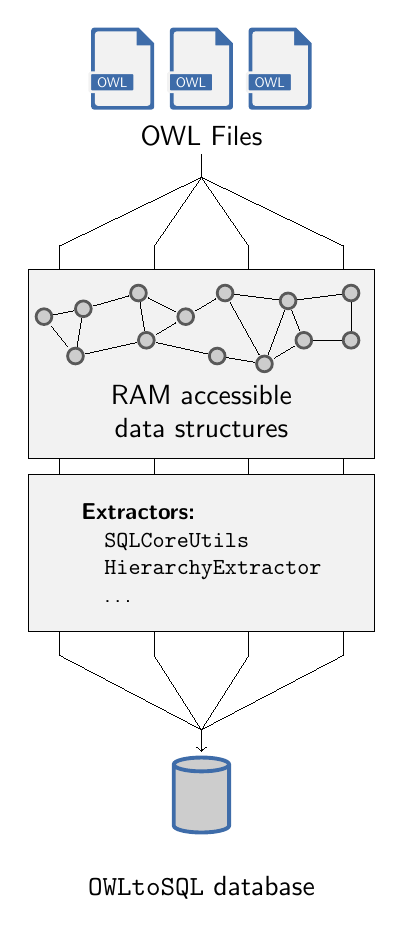
\begin{tikzpicture}[
    every node/.style={font=\sffamily},
    d/.style={fill=mygrey!30!white,line width=1pt,draw=mygrey},
    c/.style={draw=black,line width=0},
    database/.style={
        scale=3,
        draw=iconcolor,
        line width=1.4pt,
        cylinder,
        cylinder uses custom fill,
        cylinder body fill=mygrey!30,
        cylinder end fill=mygrey!30,
        shape border rotate=90,
        aspect=0.25,
        draw
    }
]

\path (-1, 0.85) pic [scale=0.8] {file};
\path ( 0, 0.85) pic [scale=0.8] {file};
\path ( 1, 0.85) pic [scale=0.8] {file};
\node (files) at (0, 0) {OWL Files};

\node [database,label={[label distance=-2cm]{\texttt{OWLtoSQL} database}}] (db) at (0, -8.5) {};

\node (r1) at (-1.8, -2) {};
\node (r2) at (-0.6, -2) {};
\node (r3) at ( 0.6, -2) {};
\node (r4) at ( 1.8, -2) {};

\node (s1) at (-1.8, -4.3) {};
\node (s2) at (-0.6, -4.3) {};
\node (s3) at ( 0.6, -4.3) {};
\node (s4) at ( 1.8, -4.3) {};

\path [c]
    (files.south) -- ++(0, -8pt) -- (-1.8, -1.4) -- (-1.8, -6.6) --
    ($(db.north)+(0,8pt)$) [->] to (db.north);
\path [c]
    (files.south) -- ++(0, -8pt) -- (-0.6, -1.4) -- (-0.6, -6.6) --
    ($(db.north)+(0,8pt)$) [->] to (db.north);
\path [c]
    (files.south) -- ++(0, -8pt) -- ( 0.6, -1.4) -- ( 0.6, -6.6) --
    ($(db.north)+(0,8pt)$) [->] to (db.north);
\path [c]
    (files.south) -- ++(0, -8pt) -- ( 1.8, -1.4) -- ( 1.8, -6.6) --
    ($(db.north)+(0,8pt)$) [->] to (db.north);

\filldraw [draw=black,fill=black!5!white]
    (-2.2,-1.7) rectangle (2.2, -4.1);
\filldraw [draw=black,fill=black!5!white]
    (-2.2,-4.3) rectangle (2.2, -6.3);

\node [align=center] at (0, -3.5) {RAM accessible\\data structures};

\def\dot (#1) (#2){\node (#1) at (#2) {}; \filldraw [d] (#1) circle (1.0mm)}

\dot (n1)  (-2.0, -2.3);
\dot (n2)  (-1.5, -2.2);
\dot (n3)  (-1.6, -2.8);
\dot (n4)  (-0.7, -2.6);
\dot (n5)  (-0.2, -2.3);
\dot (n6)  (-0.8, -2.0);
\dot (n7)  ( 0.3, -2.0);
\dot (n8)  ( 0.8, -2.9);
\dot (n9)  ( 1.3, -2.6);
\dot (n10) ( 1.1, -2.1);
\dot (n11) ( 1.9, -2.0);
\dot (n12) ( 1.9, -2.6);
\dot (n13) ( 0.2, -2.8);

\draw [line width=0] (n1) -- (n2);
\draw [line width=0] (n1) -- (n3);
\draw [line width=0] (n2) -- (n6);
\draw [line width=0] (n2) -- (n3);
\draw [line width=0] (n3) -- (n4);
\draw [line width=0] (n4) -- (n6);
\draw [line width=0] (n4) -- (n6);
\draw [line width=0] (n4) -- (n5);
\draw [line width=0] (n4) -- (n5);
\draw [line width=0] (n4) -- (n13);
\draw [line width=0] (n5) -- (n7);
\draw [line width=0] (n5) -- (n6);
\draw [line width=0] (n7) -- (n8);
\draw [line width=0] (n7) -- (n10);
\draw [line width=0] (n8) -- (n13);
\draw [line width=0] (n8) -- (n10);
\draw [line width=0] (n8) -- (n9);
\draw [line width=0] (n9) -- (n10);
\draw [line width=0] (n9) -- (n12);
\draw [line width=0] (n10) -- (n11);
\draw [line width=0] (n11) -- (n12);

\node [align=left,scale=0.83] (classes) at (0,-5.3) {%
    \textbf{Extractors:}\\%
    \hskip1em \texttt{SQLCoreUtils}\\%
    \hskip1em \texttt{HierarchyExtractor}\\%
    \hskip1em \ldots};

\end{tikzpicture}

\end{document}
